As alluded to in the previous sections, detecting communities is of great interest and as such there a number of ways to do it. The process of community detection involves analysing the network and finding groups of nodes in the network that are more densely connected amongst themselves than they are to the rest of the network. This notion forms the basis for most community detection methods and algorithms. However, a robust definition of community is difficult to formulate. In fact, it turns out that ``In most cases, communities are algorithmically defined, i.e. they are just the final product of the algorithm without a precise \emph{a priori} definition."\cite[84]{fortunato} In this section, we will discuss the notions of ``community" that underpin a number of interesting methods in community detection before going into detail about the algorithms themselves.

A simple example of the aforementioned notion comes in the form of inter and intra-cluster densities as discussed by Fortunato\cite[84]{fortunato}. This idea assumes that we have a network $N$ and a subnetwork $C \subseteq N$ i.e. $C$ is also a network where every node and edge in $C$ is also in $N$, but the converse is not necessarily true. Suppose we want to determine whether $C$ is a community inside $N$. To aid us in our investigation, we can define the following two quantities,

\begin{enumerate}
    \item Intra-cluser density: $\delta_{\text{int}}(C) = \frac{\text{\# of internal edges of C}}{n_c(n_c - 1)/2} $,
    \item Inter-cluser density: $\delta_{\text{ext}}(C) = \frac{\text{\# of external edges of C}}{n_c(n_c - 1)/2} $,
\end{enumerate}

where $n_c = |C|$ and internal and external edges refer to edges originating in $C$ that end inside and outside $C$ respectively. Thus the intra-cluster density is the ratio of edges originating in $C$ that remain in $C$ whilst the inter-cluster density is the ratio of edges originating in $C$ that end outside $C$. Finally, to make sense of these metrics, we introduce a fiducial marker for community structure, the average link density,

$$ \delta(N) = \frac{\text{\# of edges in}\; N}{n(n-1)/2}. $$

Following the same intuition as before, this quantity represents the ratio of edges that are actually present in the network agains the total number of possible edges. Now, if $C$ were a community, we would expect that $\delta_{\text{int}}(C)$ is noticeably larger than $\delta(N)$. Similarly, we would expect $\delta_{\text{ext}}(C)$ to be noticeably smaller than $\delta(N)$. Getting this result is the goal of most community detection algorithms.

Stricter definitions of communities come in three flavours: local definitions, global definitions and definitions based on vertex similarity: 

\begin{enumerate}
    \item Local definitions rely on considering the structure of a given subnetwork and perhaps it's immediately adjacent neighbours,
    \item Global definitions consider the structure of the whole network,
    \item Vertex similarity relies on the notion of similarity between any two vertices.
\end{enumerate}

Each method seeks to formalise our intuition that communities should be strongly connected amongst themselves, but weakly connected to the rest of the network. To extend this intuition, we will refer to Wasserman's summary of the four general properties of what he calls ``cohesive subgroups" (but we call communities) that have influenced the formalisations and definitions of the concept in the social network literature\cite[251-252]{wasserman_faust_1994}:

\begin{enumerate}
    \item The mutuality of ties (cliques);
    \item The closeness or reachability of subgroup (community) members;
    \item The frequency of ties amongst members (frequency of connections between community members);
    \item The relative frequency of ties amongst subgroup (community) members compared to non-subgroup (non-community) members.
\end{enumerate}

% The four points above are written in the parlance of the Social Network Analysis literature. As such, we will reprint them using terms more in line with our context:
%
% \begin{enumerate}
%     \item Cliques
%     \item Closeness or reachability of community members
%     \item Frequency of connections between community members
%     \item Relative frequency of connections amongst community members compared to non-community members.
% \end{enumerate}

Each of these points refers to a different strategy for identifying communities. Paraphrasing Wasserman and using our terminology: Strategies based on cliques require each member of a community to be directly adjacent to each other member of a community; strategies based on closeness or reachability require that each member of a community is reachable from every other member of the same community, but adjacency is not required; strategies based on frequency of connetions between community members require that each member of the community is adjacent to many other members of the community; and strategies based on the relative frequency of connections require that members of the community are more connected amongst each other than they are to the rest of the network.

These four ideas for definitions are such that the communities they generate are considered maximal subnetworks i.e. adding another node to the subnetwork would remove the subnetwork's community property. The ideas are also in decreasing order in terms of strictness and Fortunato provides an excellent summary of the journey from a rudimentary strategy using cliques to strategies involving fitness measures in the case of local definitions.\cite[88-90]{fortunato}

Global definitions, of course, follow the same notion, but they have a different motivation. Whilst local definitions are used when we're interested in just the structure of the subnetwork, global definitions are used when the community structure doesn't make sense without the context of the rest of the network and vice versa. Global definitions are more often indirect definitions in the sense that the communities are defined by the output of an algorithm implementing a global method. Curiously though, there are a set of direct global definitions. These definitions are called \emph{null model} definitions. These definitions rely on taking the original network and generating a random version of it that has some similarity in it's structural features to the original. These two networks are then compared in some way which will reveal any underlying community structure. In fact, these null model methods underpin the idea of modularity; a concept which is relied upon by the most popular method of network clustering.

\subsection{Quality Functions and Basic Modularity}\label{sec:qfs and modularity}

While considering certain dichotomies or methodological aspects is a meaningful first step, we are ultimately interested in the efficacy of a given method. Anyone can define an algorithm that breaks a network down into communities (for example by putting each node into it's own community), but some of these might not provide us with high quality insight to the structure of a network. Hence we develop the idea of \emph{quality functions}. A community detection algorihm takes a network $N$ and returns a set of partitions and/or clusters in that network based on a set of rules. A quality function determines the quality of an algorithm by assigning a number to each partition of a network. Typically, partitions with a high score are considered ``good". According to Fortunato, the most used quality function is Newman and Girvan's definition of modularity\cite[8]{newman_girvan}:

$$ Q = \sum_i (e_{ii} - a_i^2) = \text{Tr}(e) - ||e^2||. $$

This definition relies on constructing a matrix $e$ such that $e_{ij}$ is the fraction of edges in the network that link a node in community $i$ to a node in community $j$, $a_i = \sum_j e_{ij}$ the fraction of edges that connect to vertices in community $i$, and finally $||X||$ denotes the sum of all elements of the matrix $X$. Based on this definition, if our algorithm has partitioned the network successfully into communities then we expect $Q$ to be large. Even though $\text{Tr}(e)$ is large when the communities are very well connected, it achieves a maximum of $\text{Tr}(e) = 1$ when all the nodes are in the same community. This is clearly not useful as it doesn't give us any information about the structure of the networks. Thus we subtract $||e^2||$ from $\text{Tr}(e)$. To quote Newman and Girvan: ``this quantity measures the fraction of edges in the network that connect vertices of the same type minus the expecte value of the same quantity in a network with the same community divisions but with random connections between them". The idea for this definition is to use a \emph{null model} and exploit the fact that random networks are not expected to have any community strucutre.

% \subsection{Modularity}

% Note to later self: I'm kind of interested in references 77 and 78 from Fortunato's writeup. Also just generally I need to give the whole "Local definitions" thing a proper read as I'm sure there's some interesting stuff to go into there.

% In more detail, local definitions can vary a lot but the efficacy can also vary significantly. For example: cliques. Are cliques communities? Yes!

\subsection{Community Detection via Smallest Cut}\label{sec:smallest_cut}
The simplest way to consider community detection is to think about dividing the network into subnetworks such that the number of edges between all the subnetworks is minimised. This is called a smallest cut. Referring again to Lambiotte's notes, we will define a few pieces of machinery that will allow us to algorithmically find the set of edges that separates the communities\cite[26-27]{oxford:renaud_notes}. For simplicity, we restrict ourselves to trying to identify only two communities. Let us assume that we have partitioned the graph into two groups labelled 1 and 2. We then define the number of edges starting in group 1 and ending in group 2 or vice versa by the following quantity:

$$ R = \frac{1}{2} \sum_{\substack{i, j \; \text{in} \\ \text{different} \\ \text{groups}}} A_{ij}. $$

Of course, this isn't very easy to work with, so we define a vector $s$ such that

$$ s_i = 
\begin{cases}
    +1 & \text{if vertex} \; i \; \text{belongs to group 1}, \\
    -1 & \text{if vertex} \; i \; \text{belongs to group 2}. \\
\end{cases}
$$

After noting the following

$$ \frac{1}{2}(1 - s_i s_j) = 
\begin{cases}
    1 & \text{if} \; i \; \text{and} \; j \; \text{are in different groups}, \\
    0 & \text{if} \; i \; \text{and} \; j \; \text{are in the same group}, \\
\end{cases}
$$

we can rewrite $R$ as

$$
\begin{aligned}
    R =& \frac{1}{4}\sum_{ij}(1 - s_i s_j)A_{ij} \\
      =& \qquad \vdots \\
      =& \frac{1}{4}\sum_{ij}s_i s_j(k_i\delta_{ij} - A_{ij}), \\
\end{aligned}
$$

which is then equal to the following,

$$ R = \frac{1}{4}s^TLs, $$

where $L$ is the Laplacian matrix of the network. So now finding the minimum cut is equivalent to finding the vector $s$ that minimises the above quantity. The trick is to rewrite $s$ using a linear combination of the normalised eigenvectors, $v_i$ of $L$. This means that $s$ takes the form $\sum_{i=1}^n a_iv_i$ where we set $a_i = v_i^T s$. It should also be simple to see that $s^Ts = n$. Combining this redefinition of $s$ and the $a_i$s, we can note that

$$ \sum_{i=1}^n a_i^2 = n. $$

Letting $\lambda_i$ be the eigenvalue of $L$ correspnding to $v_i$, we get the following

$$ R = \sum_i a_iv_i^TL\sum_ja_jv_j = \sum_{ij}a_ia_j\lambda_j\delta{ij} = \sum{i}\lambda_i. $$

Convention dictates that we label the eigenvalues in increasing order, i.e. $\lambda_1 \leq \lambda_2 \leq \dots \leq \lambda_n$. In order to minimise the value of $R$, we wish to chose an $s$ that places as much weight on the smaller eigenvalues as possible. With this in mind, the easiest way to minimise $R$ is to choose $s = (1, 1, \dots) = v_i$ the eigenvector corresponding to $\lambda_i = \lambda_1 = 0$. This, however, is not an interesting solution as all it does is put every node into group 1 and none into group 2. To fix this, we just prohibit this solution and find the next best one. The next best solution places as much weight as possible on the second eigenvalue $\lambda_2$ of the Laplacian. To do this, we select an $s$ that is proportional to the second eigenvector, $v_2$. This eigenvector is commonly referred to the \emph{Fiedler vector}. However, due to the constraint that every $s_i = \pm 1$ we can rarely chose an $s$ that is exactly proportional to $v_2$. Lambiotte provides a more comprehensive discussion of this argument, but in this case it is often sufficient to chose $s$ as close to $v_2$ as possible. After some more algebra and manipulation, it transpires that the optimal choice for any $s_i$ under this paradigm is 

$$ s_i = \begin{cases}
    +1 & \text{if} \; v_i^{(2)} \geq 0, \\
    -1 & \text{if} \; v_i^{(2)} < 0,
\end{cases} $$

where $v_i^{(2)}$ is the $i$-th element of $v_2$. There are a few more minor issues involving constraints that are not discussed here that Lambiotte covers in good detail\cite[27]{oxford:renaud_notes}. This is perhaps the simplest method of community detection, though it is limited in its scope and power due to the fact that it can only separate the network into two groups when in reality we might be interested in $N \gg 2$ groups.

\subsection{Louvain Community Detection}
To provide some contrast, we will now explore a more advanced method known as Louvain detection, named after the University of Louvain in Belgium. Louvain detection is \emph{extremely} fast and extremely effective and operates on weighted networks as with the aforementioned Ford-Fulkerson method (Section \ref{sec:smallest_cut}). Figure \ref{fig:louvain_results_comparison} shows a comparison of the Louvain method against other contemporary methods. As you can clearly see, Louvain community detection is significantly faster than all other compared methods taking only 152 minutes to compute the community structure of a network with 118 million nodes and 1 billion edges.

\begin{figure}
    \begin{center}
        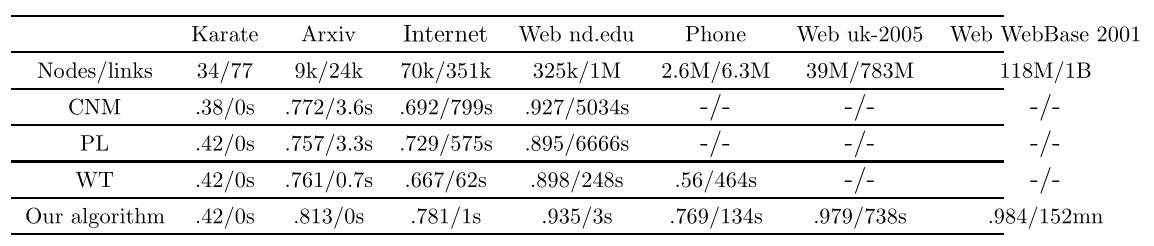
\includegraphics[width=0.95\textwidth]{img/3/comp}
    \end{center}
    \caption{A comparison of the Louvain method (noted in the table as "Our algorithm") against methods from Clauset, Newman and Moore (CNM)\cite{Clauset_2004}, Pons and Latapy (PL)\cite{JGAA-124} and Wakita and Tsurumi (WT)\cite{wakita_tsurumi}. The first row shows the number of nodes/links in each data set whilst all other rows show the modularity of the result from the algorithm and the time taken to compute the result. The symbols ``-/-" are for combinations of algorithm and dataset where the computation time was greater than 24 hours. This table is taken from \cite{Blondel_2008}.}
    \label{fig:louvain_results_comparison}
\end{figure}

\subsubsection*{Method}
The Louvain method is broken into two phases:
\begin{enumerate}
    \item Modularity optimisation;
    \item Community aggregation.
\end{enumerate}

To set up the method, we take every node in the network and put it into it's own community i.e. if there are $N$ nodes in the network then there are $N$ communities. Once we have done this, we begin phase one. In phase one we iterate over every node, $i$, in the network and consider it's neighbours, $j$. Then, for each $j$, we consider the change in modularity of the network by adding $i$ to the community that $j$ is already in. We then add $i$ in the original network to the community of $j$ that maximises the increase in modularity. Note that there must be an increase otherwise we do nothing. This process is then repeated until no single move of a vertex $i$ into the same community as $j$ increases the modularity.

Once phase one is completed, we start phase two. Phase two consists of taking all of the communities found in phase one and considering them to be nodes in a network. In this network, the links between nodes are given by the sum of the weights of edges between the respective communities and a self-link is added to every node with a weight equal to the sum of the weights of the links inside the community. We call the application of a phase one followed by a phase two a ``pass" and a diagram of this process can be seen in Figure \ref{fig:louvain_aggregation_diagram}.

\begin{figure}
    \begin{center}
        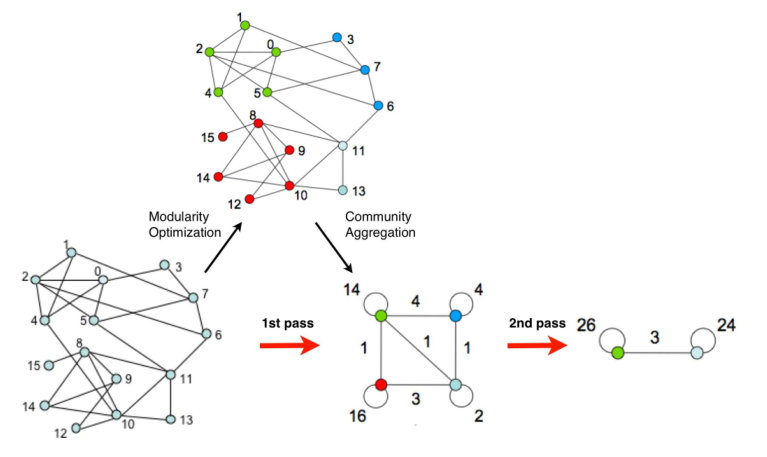
\includegraphics[width=0.95\textwidth]{img/3/louvain}
    \end{center}
    \caption{A diagram showing multiple applications of phases one and two (passes) of the Louvain algorithm from \cite{Blondel_2008}.}
    \label{fig:louvain_aggregation_diagram}
\end{figure}

\subsubsection*{Comments}
As mentioned previously, the Louvain method is extremely efficient, but where does this efficiency come from? The answer to this question is twofold. On one front, the recursive nature of the solution significantly reduces the size of the problem very quickly meaning that after the first pass, even for lager data sets, it can be very quick to find solutions. Secondly, it turns out that after some algebraic manipulation, it's very computationally cheap to calculate the change in modularity for any given move from $i$ into the community $C$:

$$ \Delta Q = \left [\frac{\Sigma_{\text{in}} + k_{i \text{in}}}{2m} - \left (\frac{\Sigma_{\text{tot}} + k_i}{2m} \right )^2 \right ] - \left [ \frac{\Sigma_{\text{in}}}{2m} - \left ( \frac{\Sigma_{\text{tot}}}{2m} \right )^2 - \left ( \frac{k_i}{2m} \right )^2\right ], $$

where $\Sigma_{\text{in}}$ is the sum of the weights of the links inside $C$, $\Sigma_{\text{tot}}$ is the sum of the weights of the lnks incident to nodes in $C$, $k_i$ is the sum o fthe weights of the links incident to the node $i$ $k_{i, \text{in}}$ is the sum of the weights of the links from $i$ to nodes in $C$ and $m$ is the sum of all the weights of all links in the network.

Louvian detection also uses a slightly different definition of modularity that is also given by Newman\cite{PhysRevE.70.056131}:

$$ Q = \frac{1}{2m} \sum_{i, j} \left [ A_{ij} - \frac{k_i k_j}{2m} \right ] \delta(c_i, c_j), $$

where $A$ is the weighted adjacency matrix for the network, $\delta$ is the Kronecker delta and $c_i$ is the community to which vertex $i$ is assigned. These two qualities, when combined, result in the extrodinary efficiency shown in Figure \ref{fig:louvain_results_comparison}
